\documentclass[12pt]{amsproc}

% a la fullpage
\usepackage{geometry}
\geometry{a4paper}
\geometry{twoside=false}

% Activate to begin paragraphs with an empty line rather than an indent
\usepackage[parfill]{parskip}
\setlength{\marginparwidth}{2cm}

\newtheorem{theorem}{Theorem}[section]
\newtheorem{definition}[theorem]{Definition}
\newtheorem{lemma}[theorem]{Lemma}

\usepackage{graphicx}
\usepackage{float}
\usepackage{amssymb}
\usepackage{color}
\usepackage{listings}

\newcommand{\id}{\text{id}}
\newcommand{\N}{\mathbb{N}}
\newcommand{\Z}{\mathbb{Z}}
\newcommand{\R}{\mathbb{R}}
\newcommand{\cat}[1]{\mathbf{#1}}
\newcommand{\Ch}[1]{\mathbf{Ch}(#1)}
\newcommand{\Hom}[3]{\mathbf{Hom}_{#1}(#2, #3)}

\newcommand{\iso}{\cong}
\newcommand{\tot}[1]{\xrightarrow{\,\,{#1}\,\,}}
\newcommand{\eps}{\varepsilon}
\newcommand{\I}{\,\mid\,}
\newcommand{\then}{\Rightarrow}
\newcommand{\inject}{\hookrightarrow}
\newcommand{\del}{\partial}
\newcommand{\nsubgrp}{\trianglelefteq}

% relative to the one who includes us :(
\graphicspath{ {../images/} }

\newcommand{\todo}[1]{
	\addcontentsline{tdo}{todo}{\protect{#1}}
	$\ast$ \marginpar{\tiny $\ast$ #1}
}
\makeatletter
	\newcommand \listoftodos{\section*{Todo list} \@starttoc{tdo}}
	\newcommand\l@todo[2]{
		\par\noindent \textit{#2}, \parbox{10cm}{#1}\par
	}
\makeatother


\title{Dold-Kan Correspondence}
\author{Joshua Moerman}

\begin{document}
\maketitle

\section{Introduction}
In this thesis we will look at a correspondence which was discovered by A. Dold and D. Kan independently, hence it is called the \emph{Dold-Kan correspondence}. Abstractly it is the following equivalence of categories:
$$ \Ch{\cat{Ab}} \simeq \cat{sAb} $$
It is interesting because objects on the left hand side are considered to be algebraic of nature, whereas objects on the right are more topological. In particular this correspondence also gives a isomorphism between homology groups (on the left hand side) and homotopy groups (on the right hand side). A bit more precise:
$$ \pi_n(A) \iso H_n(N(A)) \text{ for all } n \in \N $$
where $N: \cat{sAb} \to \Ch{\cat{Ab}}$ is one half of the equivalence.

\section{Chain Complexes}
\begin{definition}
	A chain complex $C$ is a collection of abelian groups $C_n$ together with boundary operators $\del_n: C_{n+1} \to C_n$, such that $\del_n \circ \del_{n+1} = 0$. The collections of all such objects will be denoted by $\Ch{\cat{Ab}}$.
\end{definition}

In other words a chain complex is the following diagram.
$$ \cdots \to C_4 \to C_3 \to C_2 \to C_1 \to C_0 $$

Of course we can make this more general by taking for example $R$-modules instead of abelian groups. We will later see which kind of algebraic objects make sense to use in this definition. The boundary operators give rise to certain subgroups, because all groups are abelian, subgroups are normal subgroups.

\begin{definition}
	Given a chaincomplex $C$ we define the following subgroups:
	\begin{itemize}
		\item $Z_n(C) = ker(\del: C_n \to C_{n-1}) \nsubgrp C_n$, and
		\item $B_n(C) = im(\del: C_{n+1} \to C_n) \nsubgrp C_n$.
	\end{itemize}
\end{definition}
\begin{lemma}
	Given a chaincomplex $C$ we have for all $n \in \N$:
	$$ B_n(C) \nsubgrp Z_n(C).$$
\end{lemma}
\begin{proof}
	It follows from $\del_n \circ \del_{n+1} = 0$ that $im(\del: C_{n+1} \to C_n)$ is a subset of $ker(\del: C_n \to C_{n-1})$. Those are exactly the abelian groups $B_n(C)$ and $Z_n(C)$, so $ B_n(C) \nsubgrp Z_n(C) $.
\end{proof}
\begin{definition}
	Given a chaincomplex $C$ we define the \emph{$n$-th homology group} $H_n(C)$:
	$$ H_n(C) = Z_n(C) / B_n(C).$$
\end{definition}

\subsection{The singular chaincomplex}
In order to see why we are interested in the construction of homology groups, we will look at an example from algebraic topology. We will see that homology gives a nice invariant for spaces. So we will form a chaincomplex from a topological space $X$. In order to do so, we first need some more notions.
\begin{definition}
	The topological space $\Delta^n$ is called the \emph{topological $n$-simplex} and is defined as:
	$$ \Delta^n = \{x \in \R^{n+1} \I x_i \geq 0 \text{ and } x_0 + \ldots + x_n = 1 \}.$$
	The topology on $\Delta^n$ is the subspace topology.
\end{definition}

In particular $\Delta^0$ is simply a point, $\Delta^1$ a line and $\Delta^2$ a triangle. There are nice inclusions $\Delta^n \inject \Delta^{n+1}$ which we need later on. For any $n \in \N$ we define:
\begin{definition}
	For $i \in \{0, \ldots, n+1\}$ the $i$-th face map $\delta^i : \Delta^n \inject \Delta^{n+1}$ is defined as:
	$$ \delta^i (x_0, \ldots, x_n) = (x_0, \ldots, x_{i-1}, 0, x_{i+1}, \ldots, x_n) \text{ for all } x \in \Delta^n.$$
\end{definition}

Note that if we have any continuous map $\sigma : \Delta^{n+1} \to X$ we can precompose with a face map to get $\sigma \circ \delta^i : \Delta^n \to X$. This will be used for defining the boundary operator. We can make pictures of this, and when concerning continuous maps $\sigma : \Delta^{n+1} \to X$ we will draw the images in the space $X$, instead of functions.

\todo{Make some pictures here}

\todo{Define free abelian group}

We now have enough tools to define the singular chaincomplex of a space $X$.

\begin{definition}
	For a topological space $X$ we define an abelian group $C_n(X)$ as follows.
	$$ C_n(X) = \Z[\Hom{\cat{Top}}{\Delta^n}{X}] $$
	The boundary operator $\del : C_{n+1}(X) \to C_n(X)$ is defined on generators as:
	$$ \del(\sigma) = \sigma \circ \delta^0 - \sigma \circ \delta^1 + \ldots + (-1)^{n+1} \sigma \circ \delta^{n+1}.$$
\end{definition}

This might seem a bit complicated, but we can pictures this in an intuitive way, as in figure~\ref{fig:singular_chaincomplex3}. And we see that the boundary operators really give the boundary of an $n$-simplex. To see that this indeed is a chaincomplex we have to proof that the composition of two such operators is the zero map.
\begin{figure}
	\label{fig:singular_chaincomplex3}
	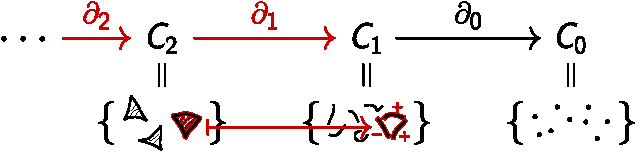
\includegraphics{singular_chaincomplex3}
	\caption{The boundary of a 2-simplex}
\end{figure}

\todo{Proposition: $C(X) \in \Ch{\cat{Ab}}$}

% \listoftodos
% \nocite{*}
% \bibliographystyle{alpha}
% \bibliography{references}	
\end{document}
